%File: formatting-instructions-latex-2024.tex
%release 2024.0
\documentclass[letterpaper]{article} % DO NOT CHANGE THIS
\usepackage{aaai24}  % DO NOT CHANGE THIS
\usepackage{times}  % DO NOT CHANGE THIS
\usepackage{helvet}  % DO NOT CHANGE THIS
\usepackage{courier}  % DO NOT CHANGE THIS
\usepackage[hyphens]{url}  % DO NOT CHANGE THIS
\usepackage{graphicx} % DO NOT CHANGE THIS
\urlstyle{rm} % DO NOT CHANGE THIS
\def\UrlFont{\rm}  % DO NOT CHANGE THIS
\usepackage{natbib}  % DO NOT CHANGE THIS AND DO NOT ADD ANY OPTIONS TO IT
\usepackage{caption} % DO NOT CHANGE THIS AND DO NOT ADD ANY OPTIONS TO IT
\frenchspacing  % DO NOT CHANGE THIS
\setlength{\pdfpagewidth}{8.5in}  % DO NOT CHANGE THIS
\setlength{\pdfpageheight}{11in}  % DO NOT CHANGE THIS
%
% These are recommended to typeset algorithms but not required. See the subsubsection on algorithms. Remove them if you don't have algorithms in your paper.
\usepackage{algorithm}
\usepackage{algorithmic}
\usepackage{amsmath,amssymb,amsfonts}
\usepackage{multirow}
%
% These are are recommended to typeset listings but not required. See the subsubsection on listing. Remove this block if you don't have listings in your paper.
\usepackage{newfloat}
\usepackage{listings}
\DeclareCaptionStyle{ruled}{labelfont=normalfont,labelsep=colon,strut=off} % DO NOT CHANGE THIS
\lstset{%
	basicstyle={\footnotesize\ttfamily},% footnotesize acceptable for monospace
	numbers=left,numberstyle=\footnotesize,xleftmargin=2em,% show line numbers, remove this entire line if you don't want the numbers.
	aboveskip=0pt,belowskip=0pt,%
	showstringspaces=false,tabsize=2,breaklines=true}
\floatstyle{ruled}
\newfloat{listing}{tb}{lst}{}
\floatname{listing}{Listing}
%
% Keep the \pdfinfo as shown here. There's no need
% for you to add the /Title and /Author tags.
\pdfinfo{
/TemplateVersion (2024.1)
}

% DISALLOWED PACKAGES
% \usepackage{authblk} -- This package is specifically forbidden
% \usepackage{balance} -- This package is specifically forbidden
% \usepackage{color (if used in text)
% \usepackage{CJK} -- This package is specifically forbidden
% \usepackage{float} -- This package is specifically forbidden
% \usepackage{flushend} -- This package is specifically forbidden
% \usepackage{fontenc} -- This package is specifically forbidden
% \usepackage{fullpage} -- This package is specifically forbidden
% \usepackage{geometry} -- This package is specifically forbidden
% \usepackage{grffile} -- This package is specifically forbidden
% \usepackage{hyperref} -- This package is specifically forbidden
% \usepackage{navigator} -- This package is specifically forbidden
% (or any other package that embeds links such as navigator or hyperref)
% \indentfirst} -- This package is specifically forbidden
% \layout} -- This package is specifically forbidden
% \multicol} -- This package is specifically forbidden
% \nameref} -- This package is specifically forbidden
% \usepackage{savetrees} -- This package is specifically forbidden
% \usepackage{setspace} -- This package is specifically forbidden
% \usepackage{stfloats} -- This package is specifically forbidden
% \usepackage{tabu} -- This package is specifically forbidden
% \usepackage{titlesec} -- This package is specifically forbidden
% \usepackage{tocbibind} -- This package is specifically forbidden
% \usepackage{ulem} -- This package is specifically forbidden
% \usepackage{wrapfig} -- This package is specifically forbidden
% DISALLOWED COMMANDS
% \nocopyright -- Your paper will not be published if you use this command
% \addtolength -- This command may not be used
% \balance -- This command may not be used
% \baselinestretch -- Your paper will not be published if you use this command
% \clearpage -- No page breaks of any kind may be used for the final version of your paper
% \columnsep -- This command may not be used
% \newpage -- No page breaks of any kind may be used for the final version of your paper
% \pagebreak -- No page breaks of any kind may be used for the final version of your paperr
% \pagestyle -- This command may not be used
% \tiny -- This is not an acceptable font size.
% \vspace{- -- No negative value may be used in proximity of a caption, figure, table, section, subsection, subsubsection, or reference
% \vskip{- -- No negative value may be used to alter spacing above or below a caption, figure, table, section, subsection, subsubsection, or reference

\setcounter{secnumdepth}{0} %May be changed to 1 or 2 if section numbers are desired.

% The file aaai24.sty is the style file for AAAI Press
% proceedings, working notes, and technical reports.
%

% Title

% Your title must be in mixed case, not sentence case.
% That means all verbs (including short verbs like be, is, using,and go),
% nouns, adverbs, adjectives should be capitalized, including both words in hyphenated terms, while
% articles, conjunctions, and prepositions are lower case unless they
% directly follow a colon or long dash
\iffalse
\title{Learning Persistent Community Structures in Dynamic Networks \\via Topological Data Analysis}
\author{
    %Authors
    % All authors must be in the same font size and format.
    Written by AAAI Press Staff\textsuperscript{\rm 1}\thanks{With help from the AAAI Publications Committee.}\\
    AAAI Style Contributions by Pater Patel Schneider,
    Sunil Issar,\\
    J. Scott Penberthy,
    George Ferguson,
    Hans Guesgen,
    Francisco Cruz\equalcontrib,
    Marc Pujol-Gonzalez\equalcontrib
}
\affiliations{
    %Afiliations
    \textsuperscript{\rm 1}Association for the Advancement of Artificial Intelligence\\
    % If you have multiple authors and multiple affiliations
    % use superscripts in text and roman font to identify them.
    % For example,

    % Sunil Issar\textsuperscript{\rm 2}, 
    % J. Scott Penberthy\textsuperscript{\rm 3}, 
    % George Ferguson\textsuperscript{\rm 4},
    % Hans Guesgen\textsuperscript{\rm 5}
    % Note that the comma should be placed after the superscript

    1900 Embarcadero Road, Suite 101\\
    Palo Alto, California 94303-3310 USA\\
    % email address must be in roman text type, not monospace or sans serif
    proceedings-questions@aaai.org
%
% See more examples next
}
\fi

%Example, Single Author, ->> remove \iffalse,\fi and place them surrounding AAAI title to use it
\iffalse
\title{My Publication Title --- Single Author}
\author {
    Author Name
}
\affiliations{
    Affiliation\\
    Affiliation Line 2\\
    name@example.com
}
\fi

%Example, Multiple Authors, ->> remove \iffalse,\fi and place them surrounding AAAI title to use it
\title{Supplementary Appendix}
\author {
    % Authors
    Dexu Kong,
    Anping Zhang,
    Yang Li\textsuperscript{\footnote{Corresponding author.}}
}
\affiliations {
    % Affiliations
    Shenzhen Key Laboratory of Ubiquitous Data Enabling, Shenzhen International Graduate School, Tsinghua University\\
    kdx21@mails.tsinghua.edu.cn,  zap21@mails.tsinghua.edu.cn, yangli@sz.tsinghua.edu.cn
}




\begin{document}

\maketitle
\appendix
\newcommand{\beginsupplement}{%
        \setcounter{table}{0}
        \renewcommand{\thetable}{S\arabic{table}}%
        \setcounter{figure}{0}
        \renewcommand{\thefigure}{S\arabic{figure}}%
     }
\renewcommand{\thealgorithm}{S\arabic{algorithm}}
\renewcommand{\figurename}{Fig.}
\beginsupplement

\section{Dataset}
We collected four labeled dynamic network datasets without node features, including Enron, Highschool \cite{crawford2018cluenet}, DBLP, Cora \cite{hou2020glodyne}. Here we introduce the detailed information of these datasets.
\begin{itemize}
    \item \textbf{Enron} dataset records the email communications of 182 employees between 2000 and 2002, with each employee having one of 7 labels representing their role in the company. The initial snapshot has 76 nodes and 161 edges, and the final snapshot has 18 nodes and 22 edges. 
    \item \textbf{Highschool} dataset corresponds to contacts between 327 students in a high school in Marseilles, France over five days, with each student having one of 9 labels representing classes. We divide one day into 10 intervals, so there are 50 snapshots in total. The initial snapshot has 279 nodes and 791 edges, and the final snapshot has 76 nodes and 80 edges. 
    \item \textbf{DBLP} dataset is a co-author network in the computer science field. The label of an author is defined by the fields in which the author has the most publications, and there are 15 labels in total. The 8 snapshots (1985-1992) are taken out to form this dynamic network. The initial snapshot has 1679 nodes and 3445 edges, and the final snapshot has 12107 nodes and 25841 edges. For \textbf{DBLP$_{dyn}$} dataset, we take 10 snapshots (2010-2019) and remove nodes with unknown labels. Note that DBLP is an accumulative network where nodes and edges do not disappear once they are added. In contrast, the coauthor communities of DBLP$_{dyn}$ appear and disappear dynamically.
% The original dataset comes from https://dblp.org/xml/release.
    \item \textbf{Cora} dataset is a citation network where each node represents a paper, and an edge between two nodes represents a citation. Each paper is assigned a label (from 10 different labels) based on its field of publication. The 11 snapshots (1989-1999) are taken out to form its dynamic network. The initial snapshot has 348 nodes and 481 edges, and the final snapshot has 12022 nodes and 45421 edges. 
\end{itemize}

\begin{table}[htbp]
\resizebox{0.48\textwidth}{!}{
\begin{tabular}{lllllll}
\hline
Dataset    & $\left| V\right|_{min}$ & $\left|E\right|_{min}$ & $\left| V\right|_{max}$  & $\left|E\right|_{max}$  & $T$  & $K$  \\ \hline
Enron      & 18   & 22   & 166   & 677   & 15 & 7  \\
Highschool & 76   & 80   & 289   & 1214  & 50 & 9  \\
Cora       & 348  & 418  & 12022 & 45421 & 11 & 10 \\
DBLP       & 1679 & 3445 & 12107 & 25841 & 8  & 15 \\
DBLP$_{dyn}$  & 2450 & 6460 & 13738 & 41934 & 10 & 14 \\ \hline
\end{tabular}
}
\caption{Dataset summary}
\label{table.dataset}
\end{table}

\section{Additional Experimental Results}
\begin{figure}[htbp] %H为当前位置,!htb为忽略美学标准,htbp为浮动图形
\centering %图片居中
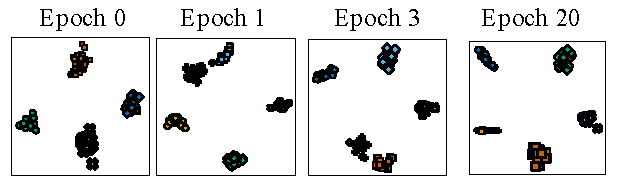
\includegraphics[width=0.48\textwidth]{pic/demo_emb_loss_v2.pdf} %插入图片,[]中设置图片大小,{}中是图片文件名
\caption{Evolution of graph embedding when Wasserstein distance of community topology between two demo graphs decreases. The colors represent the clustering results and the marker represents the ground truth labels.} %最终文档中希望显示的图片标题
\label{Fig.emb_loss_decrease} %用于文内引用的标签
\end{figure}

\begin{figure}[]
\centering %图片居中
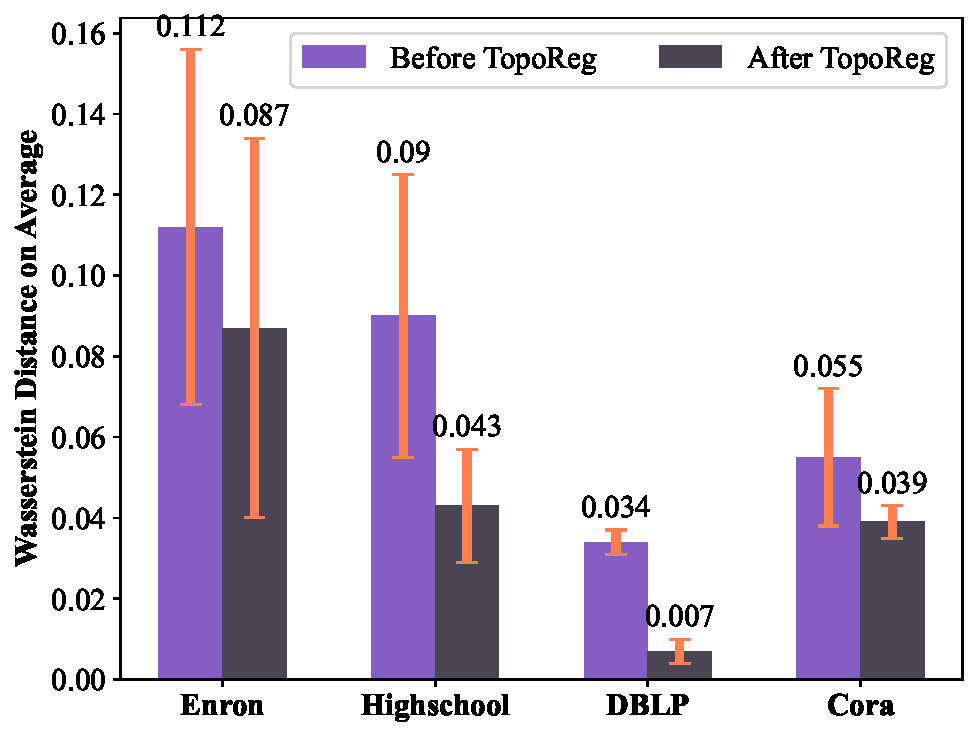
\includegraphics[width=0.45\textwidth]{pic/topo_improve.pdf} %插入图片,[]中设置图片大小,{}中是图片文件名
\caption{Wasserstein distance between community topologies in neighboring snapshots. The results prove that inter-community structure stability is improved on all four datasets after optimization using TopoReg.} %最终文档中希望显示的图片标题
\label{Fig.topoimprove} %用于文内引用的标签
\end{figure}

\noindent\textbf{Fig. \ref{Fig.emb_loss_decrease}} shows the evolution of node embedding during the training process of TopoReg. The colors represent the clustering results and the marker represents the ground truth labels. The squares and vertical crosses are initially erroneously clustered in the orange cluster, and as the epoch increases, the wasserstein distance loss decreases, and the nodes represented by the squares and crosses gradually spread out and split into two communities.

\noindent\textbf{Fig. \ref{Fig.metrics}} shows different evaluation metrics on each snapshots. The first row shows results on Highschool dataset while the second row is on Cora dataset. 
\begin{figure*}[]
\centering %图片居中
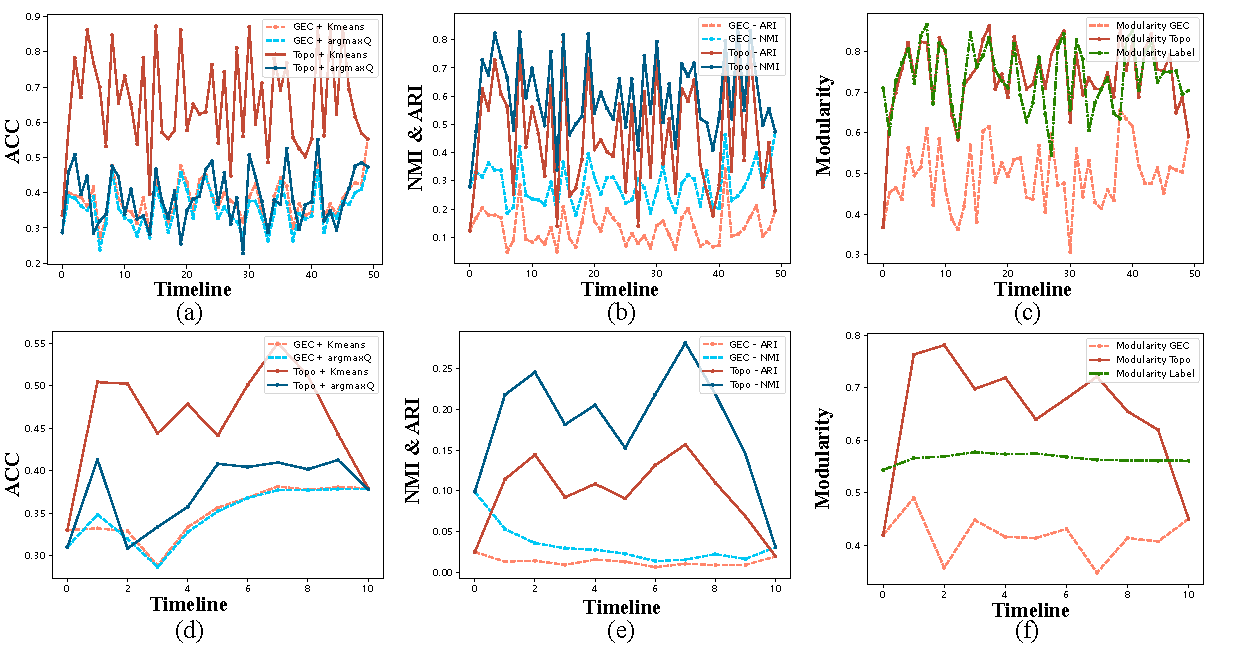
\includegraphics[width=0.95\textwidth]{pic/metrics.pdf} %插入图片,[]中设置图片大小,{}中是图片文件名
\caption{Metrics at each snapshots. The first row shows results on Highschool dataset while the second row is on Cora dataset.} %最终文档中希望显示的图片标题
\label{Fig.metrics} %用于文内引用的标签
\end{figure*}

\noindent\textbf{Fig. \ref{Fig.topoimprove}} shows the mean and standard deviation of wasserstein distance between community topologies in neighboring snapshots. It can be seen that the mean and the standard deviation have varying degrees of decreases on all four datasets. The results prove that inter-community structure stability is improved after optimization applying TopoReg.


\section{Preliminary Knowledge of Topological Data Analysis}

Topological Data Analysis (TDA) is a rising research area that uses algebraic topology concepts to analyze complex, high dimensional data. Persistent homology is the fundamental methodology in TDA that summarizes the lifetimes of topological features within a filtration as a persistence diagram. We briefly introduce it and refer the readers to \cite{dey2022computational} for more details.

\subsection{Homology}
The key concept of homology theory is to study the properties of an object \(X\), such as a \(p\)-simplex, by means of commutative algebra. A geometric \(p\)-simplex is a convex combination of \(p+1\) (affinely) independent points in \(R^N\). Complex \(K\) is a collection of simplices. A \(p\)-chain is a linear combination of \(p\)-simplices under \(\mathbb{Z}_2\)-coefficients. For a simplex \(\sigma = [x_0, \dots, x_p] \in K\), we define boundary operators as \(\partial_p(\sigma) = \sum_{i=0}^{p}[x_0, \dots , x_{i - 1}, x_{i+1}, \dots , x_p]\) and linearly extend this to chain group \(C_p(K)\), i.e. \(\partial_p( \sum \sigma_i) = \sum \partial_p(\sigma_i)\). In particular, we assign to \(K\) a sequence of chain groups \(C_0, C_1, \dots\) , which are connected by boundary operators \(\partial_n : C_n  \rightarrow C_{n-1}\) such that \(\operatorname{im} (\sigma_{n+1}) \subset \operatorname{ker} (\sigma_n)\). By studying its homology groups \(H_n = \operatorname{ker} (\sigma_n)/\operatorname{im} (\sigma_{n+1})\), we can derive topology properties of \(K\). In this case, the ranks of homology groups yield directly interpretable properties, e.g. \(rank(H_0)\) reflects the number of connected components and \(rank(H_1)\) the number of loops. We call it betti number \(\beta_p(K)=dim(H_p) = rank(Z_p)-rank(B_p)\).


% \subsection{Homology}
% The key concept of homology theory is to study the properties of an object $X$, such as a $p$-simplex, by means of commutative algebra. A geometric $p$-simplex is a convex combination of $p+1$ (affinely) independent points in $R^N$. Complex $K$ is a collection of simplices. A $p$-chain is a linear combination of $p$-simplices under $\mathbb{Z}_2$-coefficients. For a simplex $\sigma = [x_0, \dots, x_p] \in K$, we define boundary operators as $\partial_p(\sigma) = \sum_{i=0}^{p}[x_0, \dots , x_{i - 1}, x_{i+1}, \dots , x_p]$ and linearly extend this to chain group $C_p(K)$, i.e. $\partial_p( \sum \sigma_i) = \sum \partial_p(\sigma_i)$. In particular, we assign to $K$ a sequence of chain groups $C_0, C_1, \dots$ , which are connected by boundary operators $\partial_n : C_n  \rightarrow C_{n-1}$ such that $\operatorname{im} (\sigma_{n+1}) \subset \operatorname{ker} (\sigma_n)$. By studying its homology groups $H_n = \operatorname{ker} (\sigma_n)/\operatorname{im} (\sigma_{n+1})$, we can derive topology properties of $K$. In this case, the ranks of homology groups yield directly interpretable properties, e.g. $rank(H_0)$ reflects the number of connected components and $rank(H_1)$ the number of loops. We call it betti number $\beta_p(K)=dim⁡(H_p) = rank(Z_p)-rank(B_p)$. 

\subsection{Persistent Homology}
Let $\left(K^i\right)_{i=0}^m$ be a sequence of simplicial complexes such that $\emptyset=K^0 \subseteq K^1 \subseteq \cdots \subseteq K^m=K$. Then, $\left(K^i\right)_{i=0}^m$ is called a filtration of $K$. Using the extra information provided by the filtration of $K$, we obtain a sequence of chain complexes where $C_p^i=C_p\left(K_p^i\right)$. This leads to the concept of persistent homology groups, i.e.,

$$
H_p^{i, j}=\operatorname{ker} \partial_p^i /\left(\operatorname{im} \partial_{p+1}^j \cap \operatorname{ker} \partial_p^i\right) \quad \text { for } \quad 1 \leq i \leq j \leq m .
$$

The ranks, $\beta_p^{i, j} = rank(H_p^{i, j})$, of these homology groups (i.e. the $p$-th persistent Betti numbers), capture the number of homological features of dimension $p$ that persist from $i$ to (at least) $j$. we can construct a multiset by inserting the point $(a_i , a_j ), 1 \leq i < j \leq m$, with multiplicity $\mu_p^{i, j}=\left(\beta_p^{i, j-1}-\beta_p^{i, j}\right)-\left(\beta_p^{i-1, j-1}-\beta_p^{i-1, j}\right)$ . This effectively encodes the $p$-dimensional persistent homology of $K$ w.r.t. the given filtration. This representation is called a persistence barcode $B_p$, or in the form of a diagram called persistence diagram $D_p$. There are many metrics for  persistent homology, and one of them, called Wasserstein distance, is defined as the optimal transport distance between the points of the two diagrams:
\subsection{Wasserstein distance}
% \definition{1 (Wasserstein distance)}{
    For $p>0$, the $p$-Wasserstein distance between two persistence diagrams $D_k^{(1)}$ and $D_k^{(2)}$ is defined
$$
\mathrm{W}_{p, q}\left(D_k^{(1)}, D_k^{(2)}\right)=\inf _{\gamma: D_k^{(1)} \rightarrow D_k^{(2)}}\left(\sum_{x \in D_k^{(1)}}\|x-\gamma(x)\|_q^p\right)^{1 / p},
$$
    where $\|\cdot\|_q$ denotes the $q$-norm, $1 \leq q \leq \infty$ and $\gamma$ ranges over all bijections between $D_k^{(1)}$ and $D_k^{(2)}$. 
% }
% \begin{figure}[] %H为当前位置,!htb为忽略美学标准,htbp为浮动图形
% \centering %图片居中
% 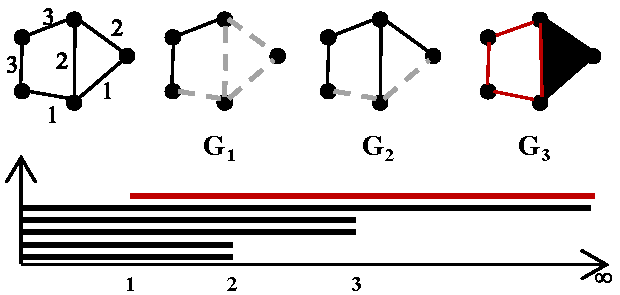
\includegraphics[width=0.45\textwidth]{wrcf.pdf} %插入图片,[]中设置图片大小,{}中是图片文件名
% \caption{Graph Filtration The process of performing weight-rank clique filtration (WRCF) on a toy graph.} %最终文档中希望显示的图片标题
% \label{Fig.wrcf} %用于文内引用的标签
% \end{figure}
\subsection{Weight Rank Clique Filtration}
Weight rank clique filtration (WRCF) \cite{petri2013topological} prioritizes the addition of edges with larger weights before those with smaller weights to emphasize the importance of edge weights. Specifically, the WRCF algorithm progressively creates unweighted graphs at each filtration step and extracts maximal cliques as simplices for further study. After obtaining a filtered complex on which we can subsequently apply persistent homology. This approach presents one of the feasible methods for applying persistent homology to temporal networks \cite{lozeve2018topological}.

\subsection{Gradient of Persistence Homology}
Substantial research advancements have been made in the field of topological optimization targeting persistence homology \cite{brüelgabrielsson2020topology,vandaele2022topologically}. Given an input filtration $f: \mathcal{X} \rightarrow$ $\mathbb{R}$, we can compute the gradient of a functional of a persistence diagram $\mathcal{E}\left(\mathrm{dgm}_k\right) =\mathcal{E}\left(\{ (b_i, d_i) \}_{i \in I_k}\right)
$ by mapping each birth-death pair to the cells that respectively created and destroyed the homology class, defining an inverse map
\begin{equation}
\label{eq:inv map}
\pi^k_f:\left\{b_i, d_i\right\}_{i \in I_k} \rightarrow(\sigma, \tau) .
\end{equation}
In the case where the ordering on simplices is strict, the map is unique, and we compute the gradient as:
\begin{equation}
\frac{\partial \mathcal{E}}{\partial \sigma}=\sum_{i \in I_k} \frac{\partial \mathcal{E}}{\partial b_i} \mathbf{1}(\pi^k_f\left(b_i\right)=\sigma)+\sum_{i \in I_k} \frac{\partial \mathcal{E}}{\partial d_i} \mathbf{1}(\pi^k_f\left(d_i\right)=\sigma)
\end{equation}
in which at most one term have a non-zero indicator. With the inverse map, we can skip the derivation of the topological calculations and directly optimize the filtration value of the corresponding simplex, which is the output of clustering module in the neural network in our method. Based on this concept, this paper extends the optimization of persistence homology to the scenario of graph filtration.

% \begin{equation*}
%     L_{\text{topo}} = \sum_{t=1}^{T-1} \sum_{k \in \{1,2\}} \left( W_{p,q} \left( dgm_k(M^{(t)}), dgm_k(M^{(t-1)}) \right) \right) + W_{p,q} \left( dgm_k(M^{(t)}), dgm_k(M^{(t+1)}) \right).

% \end{equation*}

\bibliography{supplement}

\end{document}
